\chapter{フェーズ① HTML と CSS で部のトップページをつくる}
\sheet{7-1〜7-10}

いよいよ Web ページを作ります。完成形は次のページです。
PC で見たとき（左）と、スマホで見たとき（右）で、レイアウトが変わります。

\begin{center}
\fcolorbox{gray!50}{white}{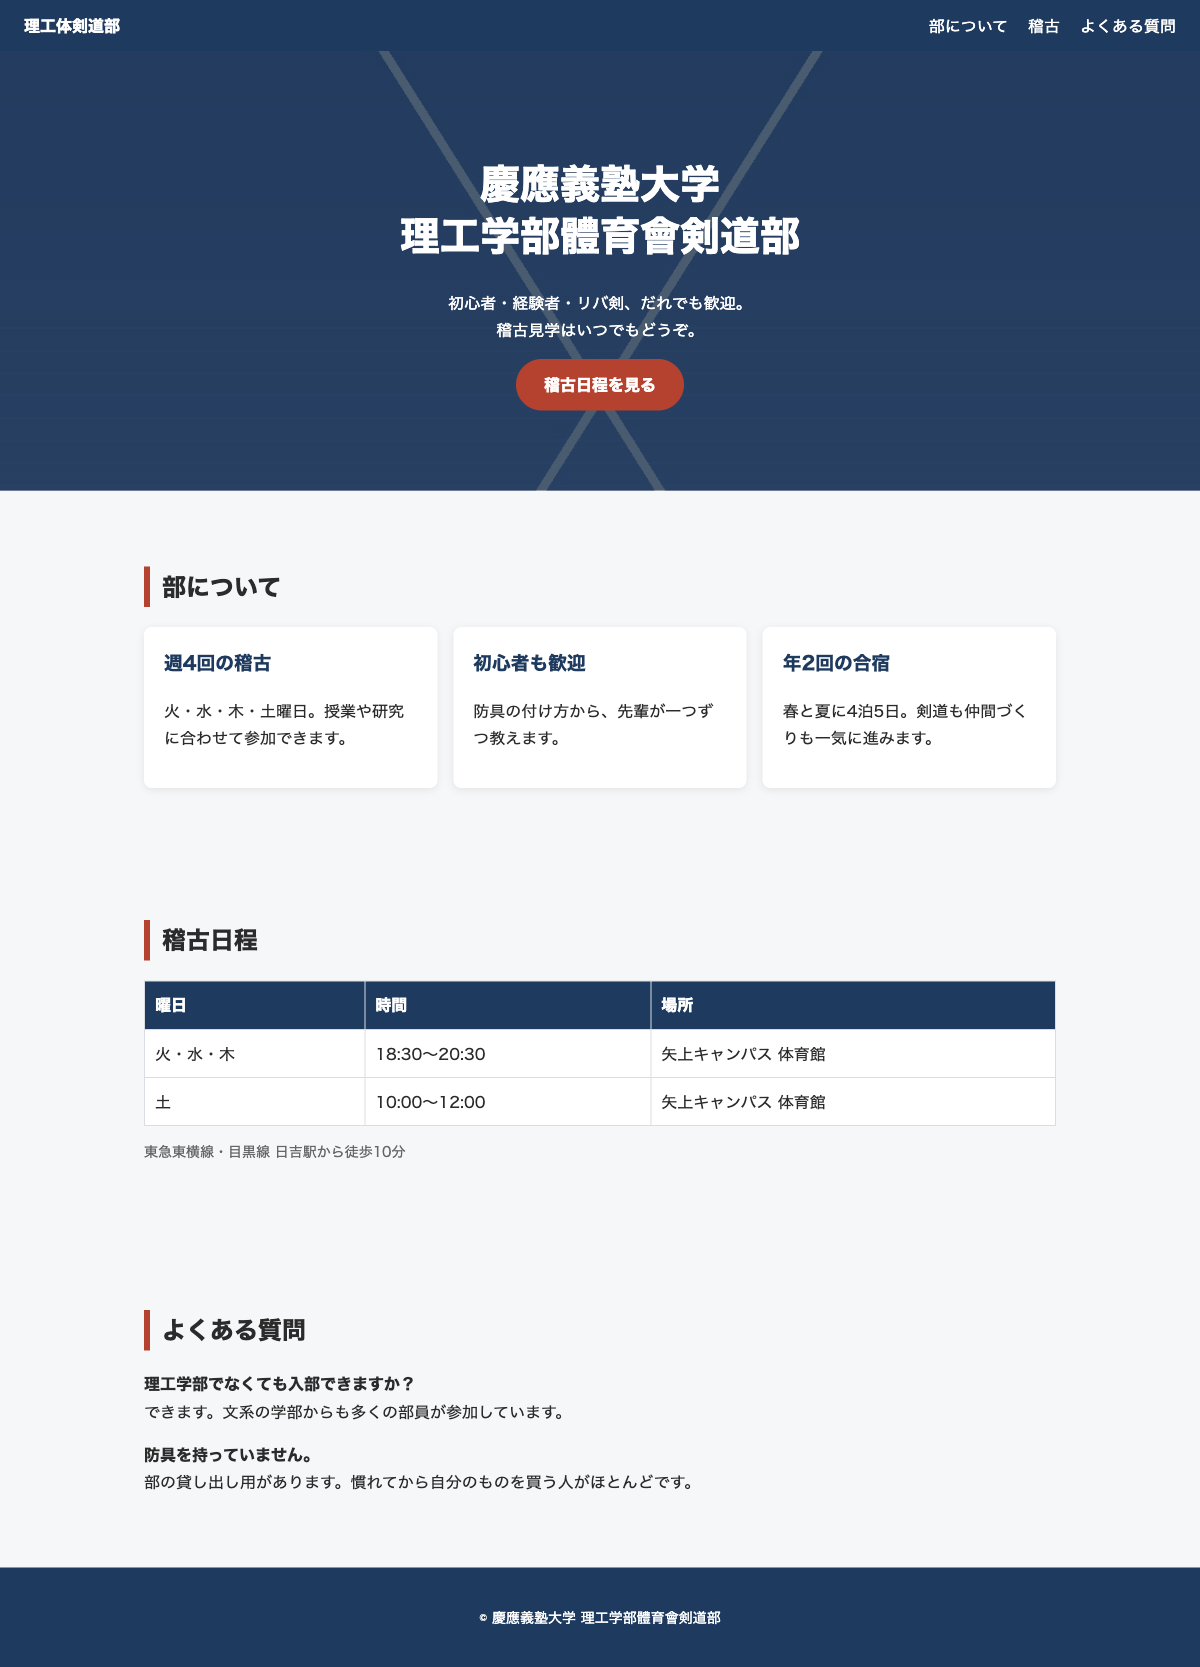
\includegraphics[width=0.58\linewidth]{kendo-top-pc.png}}\hspace{6mm}
\fcolorbox{gray!50}{white}{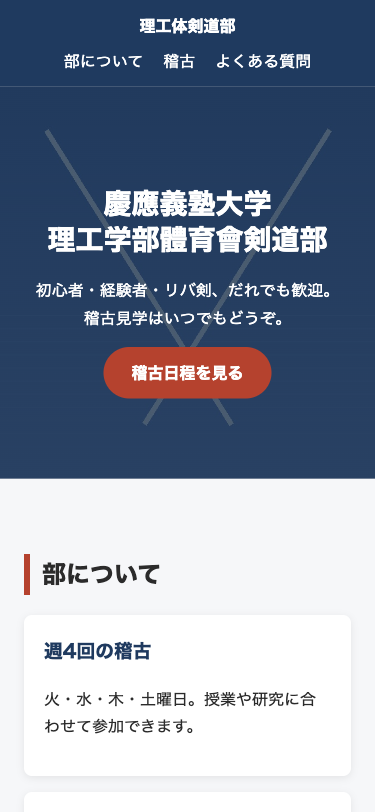
\includegraphics[width=0.25\linewidth]{kendo-top-sp.png}}
\end{center}
\figcap{完成イメージ（左：PC　右：スマホ）}

\begin{tip}[この章の進め方]
この章のコードは、\textbf{Claude に書かせず、自分の手で打ってください}。
HTML と CSS は、これから先ずっと読み書きする言葉です。一度自分の手で打っておくと、
第2巻以降で Claude が書いたコードを読むときの速さが全く違います。
打ち間違いでうまく表示されないときに原因を探すのも、大事な練習です。
\end{tip}

\section{準備：リポジトリを作る}

\begin{step}{kendo-top リポジトリを作る}
\sheet{7-1}
\begin{enumerate}
  \item GitHub で \code{kendo-top} という名前の Public リポジトリを作ります（README は Off）。
  \item 手元にフォルダを作り、Git の管理を始めます。
\end{enumerate}
\begin{terminal}[Git Bash]
$ cd ~/dev
$ mkdir kendo-top
$ cd kendo-top
$ git init
$ mkdir images
$ touch index.html style.css
$ git remote add origin git@github.com:shibayama-ryusei/kendo-top.git
$ code .
\end{terminal}
\end{step}

\begin{step}{トップ画像を用意する}
部の集合写真を三角からもらい、\code{images/hero.jpg} という名前で保存します。
\end{step}

\begin{caution}[ネットに載せてよい写真か]
このリポジトリは Public（誰でも見られる）で、GitHub Pages で公開もします。
\textbf{部員の顔が写った写真を使うときは、公開してよいものか三角に確認してください。}
本番のサイトでも、写真や名前の扱いには同じ注意が必要です。
\end{caution}

\section{HTML の骨組み}

\term{HTML} は、\term{タグ}と呼ばれる \code{<名前>} の印で文章を挟み、「ここは見出し」「ここは段落」と意味を付けていく言葉です。

\begin{center}
\begin{tikzpicture}[font=\ttfamily\small]
  \node[fill=kon!10,inner sep=3pt] (o) {<h1>};
  \node[right=0pt of o,inner sep=3pt] (t) {理工学部體育會剣道部};
  \node[right=0pt of t,fill=kon!10,inner sep=3pt] (c) {</h1>};
  \draw[<-,gray] (o.south) -- ++(0,-0.5) node[below,font=\sffamily\scriptsize]{開始タグ};
  \draw[<-,gray] (t.south) -- ++(0,-0.5) node[below,font=\sffamily\scriptsize]{中身};
  \draw[<-,gray] (c.south) -- ++(0,-0.5) node[below,font=\sffamily\scriptsize]{終了タグ（/ が付く）};
\end{tikzpicture}
\end{center}

\begin{step}{骨組みを書く}
\sheet{7-2}
\code{index.html} に次のように書きます。
\begin{filebox}{index.html}
\begin{Piton}[language=code]
<!DOCTYPE html>
<html lang="ja">
<head>
  <meta charset="UTF-8">
  <meta name="viewport" content="width=device-width, initial-scale=1.0">
  <title>慶應義塾大学 理工学部體育會剣道部</title>
  <link rel="stylesheet" href="style.css">
</head>
<body>
  <!-- ここにページの中身を書いていく -->
</body>
</html>
\end{Piton}
\end{filebox}

\begin{description}[font=\ttfamily\bfseries,style=nextline,leftmargin=2em]
  \item[<head>] ページの「設定」を書く場所。画面には表示されない
  \item[<meta charset="UTF-8">] 文字化けを防ぐおまじない。日本語を使うなら必須
  \item[<meta name="viewport" ...>] スマホで正しい幅で表示させる設定。\textbf{これがないとスマホで文字が極小になる}
  \item[<title>] ブラウザのタブに出る名前。Google の検索結果にも出る
  \item[<link rel="stylesheet" ...>] 見た目を決める CSS ファイルを読み込む
  \item[<body>] 画面に表示される中身を書く場所
  \item[<!-- -->] コメント。ブラウザは無視する。メモに使う
\end{description}
\end{step}

\section{ページを表示して確かめる}

\begin{step}{ローカルでページを開く}
\sheet{7-3}
VS Code のターミナル（\key{Ctrl}+\key{@}）で、次のように打ちます。
\begin{terminal}[Git Bash]
$ npx serve .
Need to install the following packages:
serve@14.x.x
Ok to proceed? (y) y

   ┌────────────────────────────────────────┐
   │   Serving!                             │
   │   - Local:    http://localhost:3000    │
   └────────────────────────────────────────┘
\end{terminal}
ブラウザで \url{http://localhost:3000} を開きます。真っ白なページで、タブに部の名前が出ていれば成功です。
止めるときは、ターミナルで \key{Ctrl}+\key{C} を押します。
\end{step}

\begin{why}[localhost とは]
\code{localhost} は「自分の PC」を指す特別な名前です。
\code{npx serve} は、自分の PC を小さなサーバーにして、第1章の図の「サーバー」の役をさせています。
\code{:3000} は\term{ポート番号}で、PC の中の「何番窓口か」を表します。
第2巻でサーバーの仕組みを作るときも、同じように \code{localhost} で確かめながら作ります。
\end{why}

\section{中身を書く}

\begin{step}{ヘッダーとヒーロー}
\sheet{7-4}
\code{<body>} の中のコメントを消して、次のように書きます。
\begin{filebox}{index.html（<body> の中）}
\begin{Piton}[language=code]
  <header class="site-header">
    <p class="logo">理工体剣道部</p>
    <nav>
      <ul class="nav-list">
        <li><a href="#about">部について</a></li>
        <li><a href="#practice">稽古</a></li>
        <li><a href="#faq">よくある質問</a></li>
      </ul>
    </nav>
  </header>

  <main>
    <section class="hero">
      <h1>慶應義塾大学<br>理工学部體育會剣道部</h1>
      <p>初心者・経験者・リバ剣、だれでも歓迎。<br>稽古見学はいつでもどうぞ。</p>
      <a class="button" href="#practice">稽古日程を見る</a>
    </section>

    <!-- 次の STEP で、ここにセクションを足していく -->
  </main>

  <footer class="site-footer">
    <p>&copy; 慶應義塾大学 理工学部體育會剣道部</p>
  </footer>
\end{Piton}
\end{filebox}
\end{step}

\begin{center}\small
\begin{tabularx}{\linewidth}{>{\ttfamily}l X}
\toprule
\normalfont タグ & 意味 \\
\midrule
header / main / footer & ページの頭・本体・足。意味のまとまりを示す \\
nav & サイト内の移動用メニュー \\
section & 1つの話題のまとまり \\
h1〜h6 & 見出し。数字が小さいほど大きな見出し。\textbf{h1 はページに1つ} \\
p & 段落 \\
ul / li & 箇条書きの全体／1項目 \\
a & リンク。\code{href} に行き先を書く。\code{\#about} は同じページの \code{id="about"} へ飛ぶ \\
br & 改行（終了タグなし） \\
\bottomrule
\end{tabularx}
\end{center}

\code{class="..."} は、CSS で見た目を付けるときの「名札」です。次の節で使います。

\begin{step}{部の紹介・稽古日程・よくある質問}
\sheet{7-5}
\code{<main>} の中の「次の STEP で…」のコメントを、次の3つのセクションに置き換えます。
\begin{filebox}{index.html（<main> の中、hero の下）}
\begin{Piton}[language=code]
    <section id="about" class="section">
      <h2>部について</h2>
      <div class="cards">
        <article class="card">
          <h3>週4回の稽古</h3>
          <p>火・水・木・土曜日。授業や研究に合わせて参加できます。</p>
        </article>
        <article class="card">
          <h3>初心者も歓迎</h3>
          <p>防具の付け方から、先輩が一つずつ教えます。</p>
        </article>
        <article class="card">
          <h3>年2回の合宿</h3>
          <p>春と夏に4泊5日。剣道も仲間づくりも一気に進みます。</p>
        </article>
      </div>
    </section>

    <section id="practice" class="section">
      <h2>稽古日程</h2>
      <table class="schedule">
        <tr><th>曜日</th><th>時間</th><th>場所</th></tr>
        <tr><td>火・水・木</td><td>18:30〜20:30</td><td>矢上キャンパス 体育館</td></tr>
        <tr><td>土</td><td>10:00〜12:00</td><td>矢上キャンパス 体育館</td></tr>
      </table>
      <p class="note">東急東横線・目黒線 日吉駅から徒歩10分</p>
    </section>

    <section id="faq" class="section">
      <h2>よくある質問</h2>
      <dl class="faq">
        <dt>理工学部でなくても入部できますか？</dt>
        <dd>できます。文系の学部からも多くの部員が参加しています。</dd>
        <dt>防具を持っていません。</dt>
        <dd>部の貸し出し用があります。慣れてから自分のものを買う人がほとんどです。</dd>
      </dl>
    </section>
\end{Piton}
\end{filebox}
\textbf{稽古の時間は例です。}実際の時間に書き換えてください。
\end{step}

\begin{tip}[表とリストのタグ]
\code{table}（表全体）、\code{tr}（1行）、\code{th}（見出しのマス）、\code{td}（普通のマス）。
\code{dl}・\code{dt}・\code{dd} は「用語と説明」の組で、質問と答えの組み合わせにぴったりです。
\end{tip}

ブラウザを再読み込み（\key{F5}）すると、文字だけの地味なページが表示されます。
ここまでで、一度コミットしておきましょう。

\begin{terminal}[Git Bash]
$ git add index.html images/hero.jpg
$ git commit -m "feat: トップページの HTML を作成"
\end{terminal}

\section{CSS で見た目を整える}

\term{CSS} は「どの要素に」「何を」「どうするか」を書く言葉です。

\begin{center}
\begin{tikzpicture}[font=\ttfamily\small]
  \node[fill=kon!10,inner sep=3pt] (sel) {.card};
  \node[right=2pt of sel] (b1) {\{};
  \node[right=2pt of b1,fill=kincha!15,inner sep=3pt] (prop) {color};
  \node[right=0pt of prop] (c) {:};
  \node[right=2pt of c,fill=matcha!15,inner sep=3pt] (val) {white};
  \node[right=0pt of val] (b2) {; \}};
  \draw[<-,gray] (sel.south) -- ++(0,-0.5) node[below,font=\sffamily\scriptsize,align=center]{セレクタ\\どの要素に};
  \draw[<-,gray] (prop.south) -- ++(0,-0.5) node[below,font=\sffamily\scriptsize,align=center]{プロパティ\\何を};
  \draw[<-,gray] (val.south) -- ++(0,-0.5) node[below,font=\sffamily\scriptsize,align=center]{値\\どうする};
\end{tikzpicture}
\end{center}

セレクタの書き方は、\code{.名前} で class、\code{\#名前} で id、\code{h2} のようにタグ名だけで「そのタグすべて」を指します。
\code{.section h2} のように空白で区切ると、「\code{.section} の中にある \code{h2}」という意味になります。

\begin{step}{色の約束と全体の設定}
\sheet{7-6}
\begin{filebox}{style.css}
\begin{Piton}[language=code]
/* 色の約束：ここを変えればサイト全体の色が変わる */
:root {
  --color-kon: #1f3a5f;
  --color-shu: #b5422e;
  --color-bg: #f6f7f9;
  --color-text: #2b2b2b;
}

* {
  box-sizing: border-box;
}

body {
  margin: 0;
  font-family: "Hiragino Sans", "Yu Gothic", sans-serif;
  color: var(--color-text);
  background-color: var(--color-bg);
  line-height: 1.7;
}
\end{Piton}
\end{filebox}
\code{--color-kon} は\term{CSS 変数}です。色を1か所にまとめておき、\code{var(--color-kon)} で呼び出します。
本番のサイトも、色はこうして1か所で管理しています。
\code{\#1f3a5f} は色を16進数で表したもので、赤・緑・青の強さを2桁ずつ書いています。
\end{step}

\begin{step}{ヘッダーとヒーロー}
\begin{filebox}{style.css（続き）}
\begin{Piton}[language=code]
/* ヘッダー */
.site-header {
  display: flex;
  justify-content: space-between;
  align-items: center;
  padding: 12px 24px;
  background-color: var(--color-kon);
  color: white;
}

.logo {
  margin: 0;
  font-weight: bold;
}

.nav-list {
  display: flex;
  gap: 20px;
  margin: 0;
  padding: 0;
  list-style: none;
}

.nav-list a {
  color: white;
  text-decoration: none;
}

/* ヒーロー（一番上の大きな部分） */
.hero {
  padding: 80px 24px;
  text-align: center;
  color: white;
  background: linear-gradient(rgba(31, 58, 95, 0.75), rgba(31, 58, 95, 0.75)),
    url("images/hero.jpg") center / cover;
}

.hero h1 {
  font-size: 40px;
  line-height: 1.3;
}

.button {
  display: inline-block;
  padding: 12px 28px;
  border-radius: 999px;
  background-color: var(--color-shu);
  color: white;
  text-decoration: none;
  font-weight: bold;
}
\end{Piton}
\end{filebox}
\end{step}

\section{箱の考え方：ボックスモデル}

CSS では、すべての要素を「箱」として扱います。箱は内側から順に、次の4層でできています。

\begin{center}
\begin{tikzpicture}[font=\sffamily\small]
  \draw[fill=kincha!12,draw=kincha] (0,0) rectangle (8,4.4);
  \node[anchor=north west,font=\scriptsize] at (0.1,4.35) {margin（外側の余白：となりの箱との距離）};
  \draw[fill=sumi!80,draw=sumi] (0.6,0.5) rectangle (7.4,3.8);
  \node[anchor=north west,font=\scriptsize,text=white] at (0.65,3.78) {border（枠線）};
  \draw[fill=matcha!15,draw=matcha] (0.8,0.7) rectangle (7.2,3.4);
  \node[anchor=north west,font=\scriptsize] at (0.85,3.38) {padding（内側の余白）};
  \draw[fill=white,draw=kon] (1.6,1.2) rectangle (6.4,2.8);
  \node at (4,2) {content（中身：文字や画像）};
\end{tikzpicture}
\end{center}

\code{padding: 12px 24px;} は「上下 12px、左右 24px の内側の余白」という意味です。
最初に書いた \code{box-sizing: border-box;} は、「幅を指定したら、padding と枠線もその幅の中に含める」という設定です。
これがないと、余白を足すたびに箱がはみ出していきます。

\section{横に並べる：Flexbox}

\code{display: flex;} を指定すると、その箱の\textbf{子どもたちが横一列に並びます}。
ヘッダーでロゴとメニューが左右に分かれているのは、これを使っているからです。

\begin{center}
\begin{tikzpicture}[font=\sffamily\scriptsize]
  \draw[kon,thick,rounded corners] (0,0) rectangle (9,1.2);
  \node[anchor=north west,text=kon] at (0,1.55) {\texttt{.site-header \{ display: flex; justify-content: space-between; \}}};
  \node[draw,fill=white,minimum width=2cm,minimum height=0.7cm] at (1.3,0.6) {.logo};
  \node[draw,fill=white,minimum width=3.2cm,minimum height=0.7cm] at (7.2,0.6) {nav};
  \draw[<->,shu] (2.4,0.6) -- node[above]{space-between：両端に寄せる} (5.5,0.6);
\end{tikzpicture}
\end{center}

\begin{center}\small
\begin{tabularx}{\linewidth}{>{\ttfamily}l X}
\toprule
\normalfont プロパティ & 意味 \\
\midrule
justify-content & 並ぶ方向（横）の寄せ方。\code{space-between} で両端、\code{center} で中央 \\
align-items & 並ぶ方向と直角（縦）の揃え方。\code{center} で上下中央 \\
gap & 子ども同士の間隔 \\
flex-direction & 並ぶ向き。\code{column} にすると縦に並ぶ \\
flex: 1 & （子ども側に書く）余った幅を均等に分け合う \\
\bottomrule
\end{tabularx}
\end{center}

\begin{step}{セクション・カード・表・フッター}
\sheet{7-7}
\begin{filebox}{style.css（続き）}
\begin{Piton}[language=code]
/* 各セクション共通 */
.section {
  max-width: 960px;
  margin: 0 auto;
  padding: 56px 24px;
}

.section h2 {
  border-left: 6px solid var(--color-shu);
  padding-left: 12px;
}

/* カードを横に並べる */
.cards {
  display: flex;
  gap: 16px;
}

.card {
  flex: 1;
  padding: 20px;
  background-color: white;
  border-radius: 8px;
  box-shadow: 0 2px 8px rgba(0, 0, 0, 0.08);
}

.card h3 {
  margin-top: 0;
  color: var(--color-kon);
}

/* 稽古日程の表 */
.schedule {
  width: 100%;
  border-collapse: collapse;
  background-color: white;
}

.schedule th,
.schedule td {
  padding: 10px;
  border: 1px solid #d9dde3;
  text-align: left;
}

.schedule th {
  background-color: var(--color-kon);
  color: white;
}

.note {
  font-size: 14px;
  color: #666;
}

/* よくある質問 */
.faq dt {
  font-weight: bold;
  margin-top: 16px;
}

.faq dd {
  margin-left: 0;
}

.site-footer {
  padding: 24px;
  text-align: center;
  background-color: var(--color-kon);
  color: white;
  font-size: 14px;
}
\end{Piton}
\end{filebox}
\code{max-width: 960px; margin: 0 auto;} は、「広い画面でも幅は 960px まで。左右の余白は自動で同じにする（＝中央寄せ）」という定番の書き方です。
\end{step}

\section{スマホに対応する：レスポンシブ}

このままスマホで見ると、カード3枚が横に並んだまま押しつぶされます。
画面の幅によって CSS を切り替えるのが\term{メディアクエリ}です。

\begin{step}{スマホ用の CSS を足す}
\sheet{7-8}
\begin{filebox}{style.css（一番最後に足す）}
\begin{Piton}[language=code]
/* 画面の幅が 640px 以下（スマホ）のときだけ効く */
@media (max-width: 640px) {
  .site-header {
    flex-direction: column;
    gap: 8px;
  }

  .hero h1 {
    font-size: 28px;
  }

  .cards {
    flex-direction: column;
  }
}
\end{Piton}
\end{filebox}
\end{step}

\begin{tip}[新入生はスマホで見る]
部のサイトに来る新入生のほとんどは、スマホで見ています。
作ったら\textbf{必ずスマホの幅で確かめる}ことを習慣にしてください。確かめ方は次の節で説明します。
\end{tip}

\section{開発者ツール}

ブラウザ（Chrome または Edge）で \key{F12} を押すと、\term{開発者ツール}（DevTools）が開きます。
Web 開発で一番お世話になる道具です。

\begin{center}
\begin{tikzpicture}[font=\sffamily\scriptsize]
  \draw[gray!60,fill=white] (0,0) rectangle (12,6);
  \fill[wintitle] (0,5.5) rectangle (12,6);
  \node[anchor=west] at (0.2,5.75) {localhost:3000};
  % ページ部分（スマホ表示）
  \draw[gray!50,fill=washi] (0.3,0.3) rectangle (5.6,5.3);
  \draw[kon,fill=white] (1.7,0.5) rectangle (4.2,5.1);
  \fill[kon] (1.7,4.6) rectangle (4.2,5.1);
  \node[text=white] at (2.95,4.85) {理工体剣道部};
  \fill[kon!70] (1.7,3.2) rectangle (4.2,4.6);
  \node[text=white,align=center] at (2.95,3.9) {慶應義塾大学\\理工学部…};
  \draw[gray] (1.9,2.3) rectangle (4,3.0); \draw[gray] (1.9,1.4) rectangle (4,2.1);
  \node[anchor=south] at (2.95,5.1) {\colorbox{white}{iPhone 12 Pro\ \ 390 × 844}};
  % DevTools
  \draw[gray!50,fill=white] (5.8,0.3) rectangle (11.7,5.3);
  \node[anchor=west] at (5.9,5.05) {\textbf{Elements}\quad Console\quad Sources\quad \textbf{Network}};
  \draw[shu,thick,rounded corners] (5.85,4.85) rectangle (6.95,5.25);
  \draw[gray!40] (5.8,4.8) -- (11.7,4.8);
  \node[anchor=north west,font=\ttfamily\tiny,align=left] at (5.9,4.7)
    {<header class="site-header">\\ \ \ <p class="logo">理工体剣道部</p>\\ \ \ <nav>…</nav>\\</header>\\<main>\\ \ \ <section class="hero">…};
  \draw[gray!40] (5.8,2.6) -- (11.7,2.6);
  \node[anchor=north west,font=\ttfamily\tiny,align=left] at (5.9,2.5)
    {.site-header \{\\ \ \ display: flex;\\ \ \ padding: 12px 24px;\\ \ \ background-color: \#1f3a5f;\\\}};
  % デバイス切り替えボタン
  \node[draw=shu,thick,rounded corners,fill=white] (dev) at (0.75,5.75) {\faMobile*};
  \node[anchor=west,text=shu] at (12.1,5.05) {① 要素を選ぶ};
  \node[anchor=west,text=shu] at (12.1,2.4) {② 効いている CSS};
\end{tikzpicture}
\end{center}
\figcap{開発者ツールの画面（模式図）。左上のスマホのアイコンで、スマホの幅で表示できる}

\begin{step}{開発者ツールで3つのことを試す}
\sheet{7-9}
\begin{enumerate}
  \item \textbf{スマホ表示}：\key{Ctrl}+\key{Shift}+\key{M}（またはスマホのアイコン）を押し、上の機種名から \code{iPhone SE} などを選ぶ。カードが縦に並べば、メディアクエリが効いている
  \item \textbf{要素を調べる}：左上の矢印アイコンを押してから、ページ上のボタンをクリックする。右側に、そのボタンに効いている CSS が表示される
  \item \textbf{その場で試す}：右側の CSS の値（例：\code{padding} の数字）をクリックして書き換えると、すぐに見た目に反映される。ただし\textbf{再読み込みすると元に戻る}ので、気に入ったら \code{style.css} にも書く
\end{enumerate}
\end{step}

\begin{terminal}[Git Bash]
$ git add style.css
$ git commit -m "style: トップページのデザインとスマホ対応を追加"
$ git push -u origin main
\end{terminal}

\section{GitHub Pages で公開する}

\term{GitHub Pages} を使うと、リポジトリの HTML をそのまま無料でインターネットに公開できます。

\begin{step}{Pages を有効にする}
\sheet{7-10}
\begin{enumerate}
  \item GitHub の \code{kendo-top} リポジトリを開き、\menu{Settings} → 左側の \menu{Pages} を押します。
  \item \menu{Branch} を \code{None} から \code{main} に変え、右のフォルダは \code{/ (root)} のまま \btn{Save} を押します。
\end{enumerate}
\screenshot[0.85]{github-pages-settings.jpg}
\begin{enumerate}[resume]
  \item 1〜2分待って再読み込みすると、上に \code{Your site is live at https://(ユーザー名).github.io/kendo-top/} と表示されます。
  \item そのアドレスをスマホで開いて、表示を確かめます。
\end{enumerate}
\end{step}

\begin{tip}[公開されないときのチェック]
\begin{itemize}
  \item ファイル名が \code{index.html}（すべて小文字）になっているか
  \item \code{index.html} がリポジトリの一番上の階層にあるか（フォルダの中に入っていないか）
  \item 画像が表示されないなら、ファイル名の大文字・小文字が HTML の記述と完全に一致しているか（\code{hero.JPG} と \code{hero.jpg} は別物扱い）
  \item リポジトリの \menu{Actions} タブで、\code{pages build and deployment} が緑色になっているか
\end{itemize}
\end{tip}

\section{練習問題}
\sheet{7-12〜7-27}

ここまでの内容を、手を動かして固めます。\textbf{★が多いほど難しい}問題です。
練習用に、\code{kendo-top} とは別に \code{\textasciitilde/dev/html-drill} というフォルダを作り、問題ごとに \code{q01.html}、\code{q02.html} \ldots とファイルを分けて解いてください（\code{git init} して、解けたらコミットする）。
解答例は付録にあります。\textbf{答えを見るのは、自分で書いてブラウザで確かめてから}にしてください。

\begin{tip}[練習問題での Claude の使い方]
練習問題では、Claude に答えを書かせません。使ってよいのは次の2つだけです。
\begin{itemize}
  \item 「\code{<dl>} タグの使い方を教えて。ただしこの問題の答えは書かないで」のように、\textbf{道具の使い方}を聞く
  \item 自分の答えを見せて「どこが間違っているか、ヒントだけちょうだい」と\textbf{答え合わせ}をする
\end{itemize}
\end{tip}

\subsection*{HTML}

\begin{exercise}[1]{見出しの階層}
\toanswer\par
次の文章を、\code{h1}〜\code{h3} と \code{p} を使って HTML にしてください。
\begin{quote}\small
理工体剣道部の一年（大見出し）\\
春（中見出し）\quad 新歓（小見出し）：新入生の体験稽古を行う。\quad 早慶戦（小見出し）：伝統の一戦。\\
夏（中見出し）\quad 夏合宿（小見出し）：4泊5日で鍛える。
\end{quote}
\end{exercise}

\begin{exercise}[1]{外部リンク}
\toanswer\par
「部の Instagram はこちら」という文章を書き、「こちら」を押すと \code{https://www.instagram.com/} が\textbf{新しいタブで}開くようにしてください。
新しいタブで開くときに一緒に付けるべき属性も調べて付けてください。
\end{exercise}

\begin{exercise}[1]{画像と代わりの文章}
\toanswer\par
\code{images/hero.jpg} を幅 300px で表示してください。
あわせて、画像が読み込めなかったときや、目の見えない人が読み上げソフトを使ったときに伝わる説明文を付けてください。
\end{exercise}

\begin{exercise}[2]{持ち物リスト}
\toanswer\par
「体験稽古の持ち物」として、動きやすい服装・タオル・飲み物・上履き（体育館用）の4つを箇条書きにしてください。
次に、「入部までの流れ」（見学する → 体験稽古に出る → 入部届を出す）を、\textbf{番号付き}の箇条書きにしてください。
2つでタグをどう使い分けたかを説明できるようにしておきます。
\end{exercise}

\begin{exercise}[2]{年間行事の表}
\toanswer\par
次の表を HTML で作ってください。見出しの行は \code{<thead>}、中身は \code{<tbody>} に入れます。
\begin{center}\small
\begin{tabular}{lll}\toprule
月 & 行事 & 区分 \\\midrule
4月 & 新歓・体験稽古 & イベント \\
6月 & 早慶戦 & 試合 \\
8月 & 夏合宿 & 合宿 \\
3月 & 春合宿 & 合宿 \\\bottomrule
\end{tabular}
\end{center}
\end{exercise}

\begin{exercise}[2]{間違い探し}
\toanswer\par
次の HTML には、間違いが\textbf{4つ}あります。すべて見つけて直してください。
\begin{filebox}{q06.html}
\begin{Piton}[language=code]
<section>
  <h2>稽古について<h2>
  <p>稽古は<strong>週4回</p></strong>
  <ul>
    <p>火曜日</p>
    <li>水曜日</li>
  </ul>
  <img src="images/hero.jpg">
</section>
\end{Piton}
\end{filebox}
\end{exercise}

\begin{exercise}[2]{問い合わせフォーム（見た目だけ）}
\toanswer\par
名前・メールアドレス・問い合わせ内容（複数行）・送信ボタンの4つを持つフォームを作ってください。
\begin{itemize}
  \item 各入力欄には \code{<label>} を付け、ラベルを押すとその入力欄にカーソルが入るようにする
  \item メールアドレス欄は、メールの形になっていないと送信できないようにする
  \item 名前とメールアドレスは、空のままでは送信できないようにする
\end{itemize}
（実際の送信の仕組みは第5巻で作ります。ここでは見た目と入力のチェックだけです。）
\end{exercise}

\subsection*{CSS}

\begin{exercise}[1]{サイトの色を一気に変える}
\toanswer\par
\code{kendo-top} の \code{style.css} で、\textbf{\code{:root} の中だけを書き換えて}、紺の部分を深緑（\code{\#1e4d3a}）に、朱の部分を金色（\code{\#b8860b}）に変えてください。
確かめたら、\code{git restore style.css} で元に戻します。
CSS 変数を使うと何がうれしいのかを、1文で説明できるようにしておきます。
\end{exercise}

\begin{exercise}[1]{セレクタはどれに効く？}
\toanswer\par
次の HTML と CSS で、\textbf{赤くなる文字}はどれでしょう。ブラウザで確かめる前に予想を書いてください。
\begin{filebox}{q09.html}
\begin{Piton}[language=code]
<section class="news">
  <h2>お知らせ</h2>
  <p>新歓稽古を行います。</p>
  <p class="important">雨天でも実施します。</p>
</section>
<p class="important">このサイトは練習用です。</p>

<style>
  .news p { color: red; }
  #top { color: red; }
  h3 { color: red; }
</style>
\end{Piton}
\end{filebox}
\end{exercise}

\begin{exercise}[2]{箱の幅を計算する}
\toanswer\par
次の CSS が付いた \code{div} の、\textbf{画面上での横幅}（枠線の外側まで）は何 px でしょう。
(1) \code{box-sizing} の指定がない場合と、(2) \code{box-sizing: border-box;} がある場合の両方を計算し、
開発者ツールで実際の数字を確かめてください。
\begin{Piton}[language=code]
div { width: 300px; padding: 20px; border: 2px solid black; margin: 10px; }
\end{Piton}
\end{exercise}

\begin{exercise}[2]{ボタンに反応をつける}
\toanswer\par
\code{.button} にマウスを乗せたとき、少し暗い色になり、0.2秒かけてなめらかに色が変わるようにしてください。
（ヒント：\code{:hover} と \code{transition}）
\end{exercise}

\begin{exercise}[2]{フッターを3列にする}
\toanswer\par
フッターを、「部の名前」「稽古場所」「SNS」の3つのかたまりが横に並ぶ形に作り変えてください。
スマホの幅では縦1列に並ぶようにします。
\end{exercise}

\begin{exercise}[3]{どちらの CSS が勝つ？}
\toanswer\par
次の3つのルールが同じ \code{<h2 class="title" id="main-title">} に当たったとき、文字は何色になるでしょう。
理由を「詳細度」という言葉を使って説明してください。
\begin{Piton}[language=code]
#main-title { color: green; }
h2.title    { color: blue; }
.title      { color: red; }
\end{Piton}
そのうえで、3つ目の \code{.title} の色を勝たせるにはどう書き換えればよいかを考えてください（\code{!important} は使わない）。
\end{exercise}

\subsection*{レスポンシブと開発者ツール}

\begin{exercise}[2]{タブレットでは2列にする}
\toanswer\par
「部について」のカードを、画面の幅に応じて次のように並べてください。
\begin{center}\small
\begin{tabular}{ll}\toprule
画面の幅 & カードの並び \\\midrule
961px 以上（PC） & 横に3枚 \\
641〜960px（タブレット） & 2枚ずつ（3枚目は次の行） \\
640px 以下（スマホ） & 縦に1枚ずつ \\\bottomrule
\end{tabular}
\end{center}
（ヒント：\code{flex-wrap: wrap;} と、カードの幅の指定）
\end{exercise}

\begin{exercise}[2]{開発者ツールで原因を探す}
\toanswer\par
\code{kendo-top} の見出し（\code{h2}）の左にある朱色の線について、開発者ツールだけを使って次のことを調べてください。
\begin{enumerate}
  \item その線は、\code{style.css} の何行目の、どのプロパティで指定されているか
  \item 線の太さを開発者ツール上で 12px に変えると、どう見えるか
  \item 再読み込みすると元に戻ることを確かめる
\end{enumerate}
\end{exercise}

\begin{exercise}[3]{見本を再現する}
\toanswer\par
次の見本と同じ見た目の「部の数字」セクションを、HTML と CSS で作ってください。
数字は大きく朱色、説明は小さく灰色です。スマホでは2枚ずつ並べます。
\begin{center}
\begin{tikzpicture}[font=\sffamily]
  \draw[gray!30,fill=washi] (-0.3,-0.4) rectangle (12.3,2.2);
  \foreach \x/\n/\t in {0/52/部員数,3.1/4/週の稽古回数,6.2/2/年間の合宿,9.3/70/初心者・リバ剣の割合（\%）}{
    \draw[fill=white,draw=gray!20,rounded corners=4pt] (\x,0) rectangle (\x+2.8,1.8);
    \node[text=shu,font=\sffamily\bfseries\huge] at (\x+1.4,1.15) {\n};
    \node[text=gray,font=\sffamily\scriptsize] at (\x+1.4,0.4) {\t};
  }
\end{tikzpicture}
\end{center}
（数字はダミーです）
\end{exercise}


\begin{challenge}{「大会結果」のセクションを足す}
\sheet{7-28}
次の条件で、「稽古日程」と「よくある質問」の間に「最近の大会結果」セクションを追加してください。
\begin{enumerate}
  \item 大会名・日付・結果の3列の表にする（内容はダミーでよい。例：「関東理工科大学剣道大会　2026年10月　団体戦 ベスト8」を3行）
  \item ヘッダーのメニューにも「大会結果」を足し、押すとそのセクションに飛ぶ
  \item \textbf{スマホの幅で見たときに、表がはみ出して画面全体が横にずれないこと}（ヒント：表を \code{div} で囲み、その \code{div} に \code{overflow-x: auto;} を付ける）
  \item 1つの意味ごとにコミットして push し、GitHub Pages で確かめる
\end{enumerate}
\textbf{手を動かす前に}、「どのファイルの、どこに、何を足すか」をスプシの詰まりメモ欄に箇条書きで書いてください。
終わったら、書いたメモと実際にやったことがどう違ったかを、定例で説明します。
\end{challenge}

\begin{checklist}
\begin{itemize}
  \checkitem \code{<head>} と \code{<body>} の役割の違いを言える
  \checkitem class と id の使い分けを説明できる
  \checkitem CSS のセレクタ・プロパティ・値を指して説明できる
  \checkitem ボックスモデルの4層（margin・border・padding・content）を図で描ける
  \checkitem Flexbox で要素を横に並べられる
  \checkitem メディアクエリでスマホ用の見た目を切り替えられる
  \checkitem 開発者ツールで、要素に効いている CSS を調べられる
  \checkitem GitHub Pages で公開し、スマホで確かめた
\end{itemize}
\end{checklist}
